\documentclass[10pt]{article}

\usepackage[a4paper,margin=0.65in]{geometry}
\usepackage{amsmath,amssymb}
\usepackage{graphicx}
\usepackage{booktabs}
\usepackage{array}
\usepackage{float}
\usepackage{hyperref}
\usepackage{enumitem}
\usepackage{xcolor}

\setlist{nosep,leftmargin=*}
\renewcommand{\arraystretch}{1.2}
\setlength{\parindent}{0pt}
\setlength{\parskip}{2pt}

\begin{document}

%%%%%%%%%%%%%%%%%%%%%%%%%%%%%%%%%%%%%%%%%%%%%%%%%%%%%%%%%%%%
% TITLE
%%%%%%%%%%%%%%%%%%%%%%%%%%%%%%%%%%%%%%%%%%%%%%%%%%%%%%%%%%%%

\begin{center}

{\large\textbf{Shiv Nadar University Chennai}}

\vspace{2mm}

{\normalsize\textbf{CS3807 -- Deep Learning Laboratory}}

\vspace{2mm}

{\large\textbf{Experiment 7}}

\vspace{1mm}

{\normalsize\textbf{End-to-End Study of Autoencoders, Convolutional}}

{\normalsize\textbf{Autoencoders, Denoising Autoencoders and Variational Autoencoders}}

\end{center}

\vspace{3mm}

\begin{tabular}{|p{3.4cm}|p{9.0cm}|p{1.4cm}|}
\hline
Degree \& Branch &
B.Tech Artificial Intelligence \& Data Science &
Semester V\\
\hline
Subject Code \& Name &
CS3807 -- Deep Learning Laboratory &
AY: 2026--27\\
\hline
\end{tabular}

\vspace{4mm}

%%%%%%%%%%%%%%%%%%%%%%%%%%%%%%%%%%%%%%%%%%%%%%%%%%%%%%%%%%%%
\section{Objective}
%%%%%%%%%%%%%%%%%%%%%%%%%%%%%%%%%%%%%%%%%%%%%%%%%%%%%%%%%%%%

The objective of this experiment is to develop an end-to-end understanding of autoencoders and their
variants for image representation, reconstruction, denoising and generative modeling. Starting from a
fully connected autoencoder, the experiment progresses to a Convolutional Autoencoder (CAE), introduces
controlled image corruption for a denoising autoencoder, and finally implements a Variational Autoencoder
(VAE). The learned latent representations are visualized, reconstruction quality is compared using MSE,
MAE and SSIM, and the generative capability of the VAE is explored through sampling and latent
interpolation. All four models were trained under a controlled protocol on the same MNIST subset.

%%%%%%%%%%%%%%%%%%%%%%%%%%%%%%%%%%%%%%%%%%%%%%%%%%%%%%%%%%%%
\section{Learning Outcomes}
%%%%%%%%%%%%%%%%%%%%%%%%%%%%%%%%%%%%%%%%%%%%%%%%%%%%%%%%%%%%

\begin{itemize}
\item Explain the encoder--latent--decoder structure of an autoencoder.
\item Prepare image data for reconstruction-based learning.
\item Implement a fully connected autoencoder and a Convolutional Autoencoder.
\item Introduce controlled noise and build a denoising autoencoder.
\item Evaluate reconstruction using MSE, MAE and SSIM.
\item Visualize and interpret latent representations.
\item Implement the VAE reparameterization trick and interpret reconstruction/KL losses.
\item Generate new images by sampling from a learned latent space.
\item Compare deterministic and variational latent representations.
\end{itemize}

%%%%%%%%%%%%%%%%%%%%%%%%%%%%%%%%%%%%%%%%%%%%%%%%%%%%%%%%%%%%
\section{Dataset and Experimental Setup}
%%%%%%%%%%%%%%%%%%%%%%%%%%%%%%%%%%%%%%%%%%%%%%%%%%%%%%%%%%%%

The MNIST Handwritten Digit Dataset was used, loaded directly via
\texttt{tensorflow.keras.datasets.mnist}. Each image has spatial dimensions $28\times28\times1$.
As recommended for the laboratory execution, a fixed subset of \textbf{10{,}000 training images} and
\textbf{2{,}000 test images} was randomly sampled (seed = 42) from the full 60{,}000/10{,}000 MNIST
split. Labels were used only for latent-space visualization and were never supplied as reconstruction
targets. Pixel values were normalized from $[0,255]$ to $[0,1]$.

\begin{center}
\begin{tabular}{|l|r|}
\hline
\textbf{Property} & \textbf{Value}\\
\hline
Full training samples & 60{,}000\\
Full test samples & 10{,}000\\
Selected training samples & 10{,}000\\
Selected test samples & 2{,}000\\
Image shape & $28\times28\times1$\\
Flattened vector length & 784\\
Normalized pixel range & $[0.00,\,1.00]$\\
Number of classes & 10\\
Device used & GPU (T4)\\
\hline
\end{tabular}
\end{center}

\begin{figure}[H]
\centering
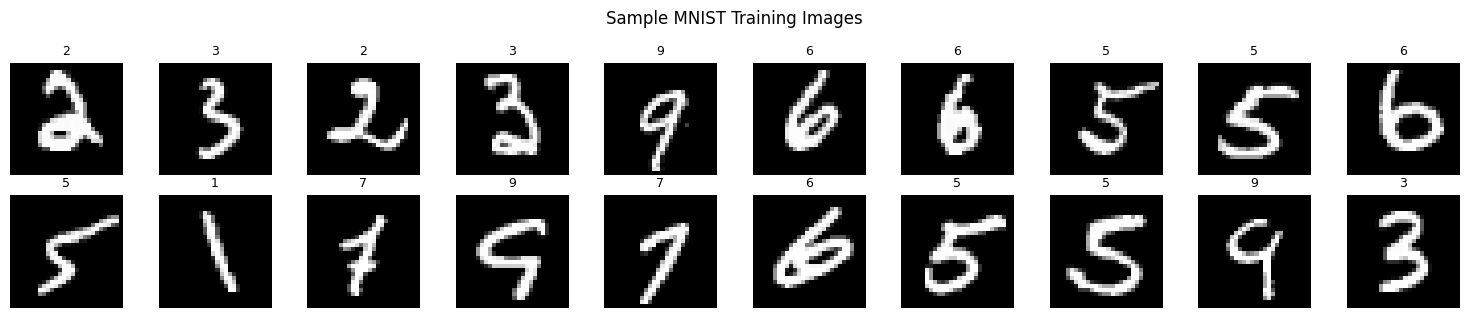
\includegraphics[width=0.85\linewidth]{images/sample_images.png}
\caption{Sample MNIST training images from the selected subset.}
\label{fig:samples}
\end{figure}

%%%%%%%%%%%%%%%%%%%%%%%%%%%%%%%%%%%%%%%%%%%%%%%%%%%%%%%%%%%%
\section{Expected Input and Output}
%%%%%%%%%%%%%%%%%%%%%%%%%%%%%%%%%%%%%%%%%%%%%%%%%%%%%%%%%%%%

For the fully connected autoencoder, each image is flattened to $x \in \mathbb{R}^{784}$. For the
convolutional, denoising and variational models, the spatial structure is retained as
$x \in \mathbb{R}^{28\times28\times1}$. In every case the output is a reconstructed image
$\hat{x} \in \mathbb{R}^{28\times28\times1}$ (or its flattened equivalent). For the denoising model the
output additionally includes the noisy input, and for the VAE the output additionally includes newly
generated samples obtained by decoding vectors drawn from the latent prior.

%%%%%%%%%%%%%%%%%%%%%%%%%%%%%%%%%%%%%%%%%%%%%%%%%%%%%%%%%%%%
\section{Overall Experimental Pipeline}
%%%%%%%%%%%%%%%%%%%%%%%%%%%%%%%%%%%%%%%%%%%%%%%%%%%%%%%%%%%%

\begin{center}
\textbf{MNIST $\rightarrow$ Normalization $\rightarrow$ Encoder $\rightarrow$ Latent Representation
$\rightarrow$ Decoder $\rightarrow$ Reconstructed Image $\rightarrow$ Evaluation}
\end{center}

The experiment consists of four related studies executed in sequence: (1) Fully Connected Autoencoder,
(2) Convolutional Autoencoder, (3) Denoising Convolutional Autoencoder, and (4) Variational Autoencoder,
followed by a latent-dimension study and eight additional exercises.

%%%%%%%%%%%%%%%%%%%%%%%%%%%%%%%%%%%%%%%%%%%%%%%%%%%%%%%%%%%%
\section{Exploring Autoencoders}
%%%%%%%%%%%%%%%%%%%%%%%%%%%%%%%%%%%%%%%%%%%%%%%%%%%%%%%%%%%%

An autoencoder learns to reproduce its input at its output. The encoder maps the input to a
lower-dimensional latent representation $z = f_\theta(x)$, and the decoder reconstructs the input
$\hat{x} = g_\phi(z)$. The training objective minimizes reconstruction error:
\[
\mathcal{L}_{rec} = \frac{1}{N}\sum_{i=1}^{N} \lVert x_i - \hat{x}_i \rVert^2 .
\]
The latent vector $z$ is a compressed representation of the input image and forms the bottleneck through
which all information relevant to reconstruction must pass.

%%%%%%%%%%%%%%%%%%%%%%%%%%%%%%%%%%%%%%%%%%%%%%%%%%%%%%%%%%%%
\section{Fully Connected Autoencoder}
%%%%%%%%%%%%%%%%%%%%%%%%%%%%%%%%%%%%%%%%%%%%%%%%%%%%%%%%%%%%

The FC-AE follows the architecture $784 \rightarrow 128 \rightarrow 32 \rightarrow 16\text{(latent)}
\rightarrow 32 \rightarrow 128 \rightarrow 784$, with ReLU activations in the hidden layers and a
sigmoid output activation. It was trained with the Adam optimizer (learning rate $10^{-3}$), batch size
128, for 20 epochs, using Binary Cross-Entropy loss.

\begin{center}
\begin{tabular}{|l|r|}
\hline
\textbf{Parameter} & \textbf{Value}\\
\hline
Latent dimension & 16\\
Trainable parameters & 211{,}040\\
Optimizer & Adam ($\eta=10^{-3}$)\\
Batch size & 128\\
Epochs & 20\\
Training time & 13.61 s\\
Final training loss (BCE) & 0.12984\\
Final validation loss (BCE) & 0.12939\\
\hline
\end{tabular}
\end{center}

%%%%%%%%%%%%%%%%%%%%%%%%%%%%%%%%%%%%%%%%%%%%%%%%%%%%%%%%%%%%
\section{Required Analysis of the Basic Autoencoder}
%%%%%%%%%%%%%%%%%%%%%%%%%%%%%%%%%%%%%%%%%%%%%%%%%%%%%%%%%%%%

\begin{figure}[H]
\centering
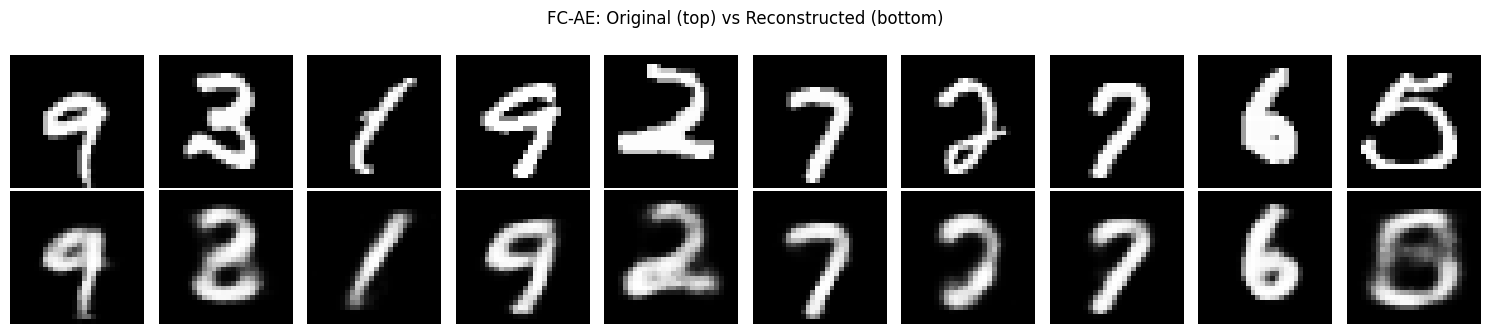
\includegraphics[width=0.9\linewidth]{images/plot1.png}
\caption{FC-AE: original (top row) versus reconstructed (bottom row) test images.}
\label{fig:plot1}
\end{figure}

The overall digit shape is preserved for every sample, but the reconstructions are visibly blurred and
fine strokes are smoothed out. Thin, cursive-style digits (e.g.\ the 1 and 2) lose sharp edges, and the
last sample (a genuine 5) is reconstructed with an ambiguous loop that resembles an 8 -- a difficult case
where flattening the image discards the spatial cues that would otherwise disambiguate the stroke. Easy,
well-separated digits such as 7 and 9 reconstruct considerably more cleanly than digits with overlapping
or curved strokes.

\begin{figure}[H]
\centering
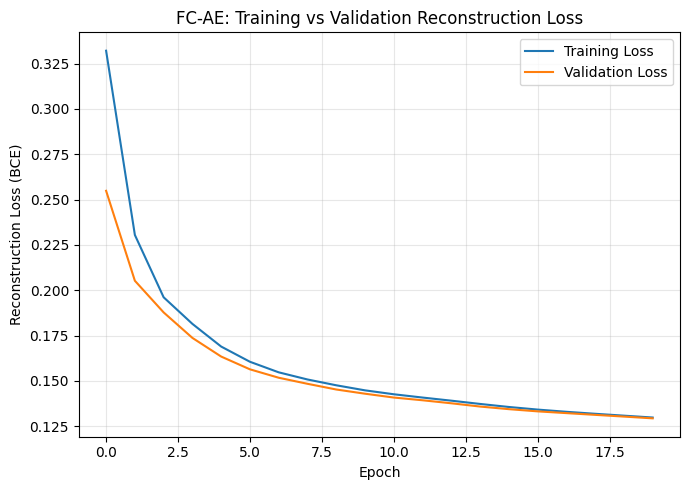
\includegraphics[width=0.65\linewidth]{images/plot2.png}
\caption{FC-AE training and validation reconstruction loss over 20 epochs.}
\label{fig:plot2}
\end{figure}

Both curves decrease smoothly and converge to nearby values (final training loss 0.12984, final
validation loss 0.12939, a gap of only 0.00045), indicating stable convergence with no sign of
overfitting on this subset.

%%%%%%%%%%%%%%%%%%%%%%%%%%%%%%%%%%%%%%%%%%%%%%%%%%%%%%%%%%%%
\section{Reconstruction Metrics}
%%%%%%%%%%%%%%%%%%%%%%%%%%%%%%%%%%%%%%%%%%%%%%%%%%%%%%%%%%%%

\begin{center}
\begin{tabular}{|l|r|}
\hline
\textbf{Metric} & \textbf{Value}\\
\hline
Test MSE & 0.022270\\
Test MAE & 0.059194\\
Mean SSIM & 0.745986\\
\hline
\end{tabular}
\end{center}

%%%%%%%%%%%%%%%%%%%%%%%%%%%%%%%%%%%%%%%%%%%%%%%%%%%%%%%%%%%%
\section{Convolutional Autoencoder}
%%%%%%%%%%%%%%%%%%%%%%%%%%%%%%%%%%%%%%%%%%%%%%%%%%%%%%%%%%%%

The CAE follows \texttt{Conv2D(32)$\to$MaxPool$\to$Conv2D(64)$\to$MaxPool$\to$Conv2D(64)$\to$UpSampling
$\to$Conv2D(32)$\to$UpSampling$\to$Conv2D(1,sigmoid)}, trained under the identical protocol as the FC-AE
(Adam, $\eta=10^{-3}$, batch size 128, 20 epochs, BCE loss) for a controlled comparison.

\begin{center}
\begin{tabular}{|l|r|}
\hline
\textbf{Parameter} & \textbf{Value}\\
\hline
Trainable parameters & 74{,}497\\
Training time & 24.31 s\\
Final training loss (BCE) & 0.06843\\
Final validation loss (BCE) & 0.06786\\
Test MSE & 0.002419\\
Test MAE & 0.014711\\
Mean SSIM & 0.975349\\
\hline
\end{tabular}
\end{center}

%%%%%%%%%%%%%%%%%%%%%%%%%%%%%%%%%%%%%%%%%%%%%%%%%%%%%%%%%%%%
\section{Comparing Fully Connected and Convolutional Autoencoders}
%%%%%%%%%%%%%%%%%%%%%%%%%%%%%%%%%%%%%%%%%%%%%%%%%%%%%%%%%%%%

\begin{center}
\begin{tabular}{|l|r|r|r|r|}
\hline
\textbf{Model} & \textbf{MSE} & \textbf{MAE} & \textbf{SSIM} & \textbf{Parameters}\\
\hline
Fully Connected AE & 0.02227 & 0.05919 & 0.74599 & 211{,}040\\
Convolutional AE & 0.00242 & 0.01471 & 0.97535 & 74{,}497\\
\hline
\end{tabular}
\end{center}

\begin{figure}[H]
\centering
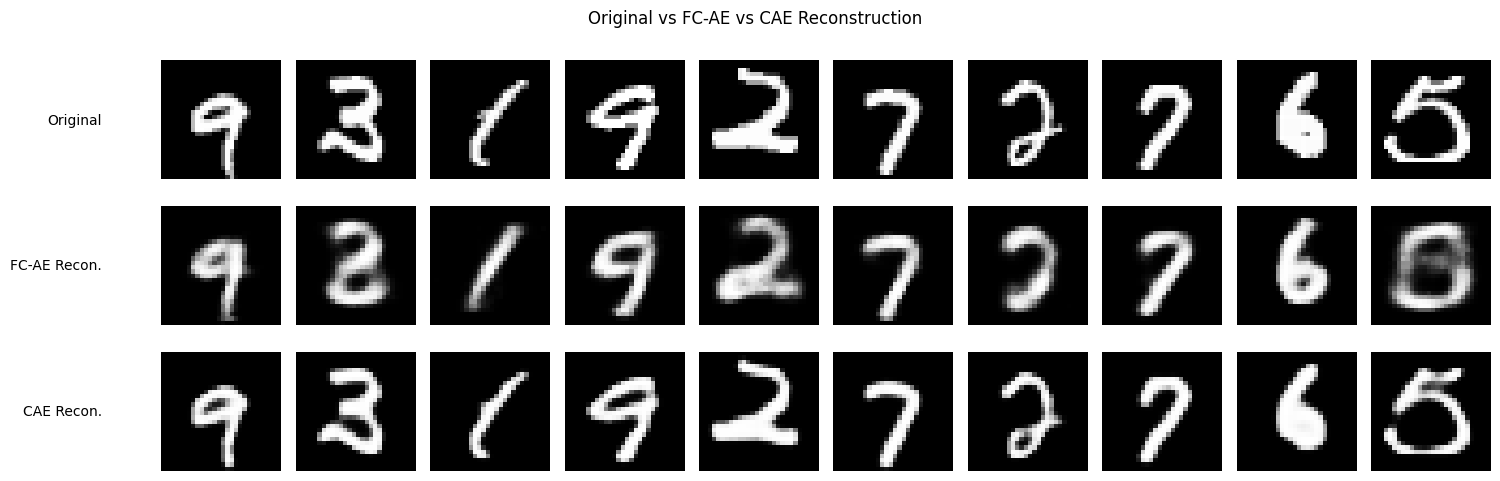
\includegraphics[width=0.9\linewidth]{images/plot3.png}
\caption{Original versus FC-AE reconstruction versus CAE reconstruction on the same test samples.}
\label{fig:plot3}
\end{figure}

The CAE achieves roughly a 9-fold lower MSE and a 15-percentage-point higher SSIM than the FC-AE while
using \emph{fewer} parameters (74{,}497 versus 211{,}040). By preserving spatial locality through
convolution and pooling instead of flattening the image into a vector, the CAE retains stroke geometry
and edges far more faithfully -- visible directly in Figure~\ref{fig:plot3}, where the CAE reconstructions are sharper
and the ambiguous 5$\to$8 confusion seen in the FC-AE disappears entirely.

%%%%%%%%%%%%%%%%%%%%%%%%%%%%%%%%%%%%%%%%%%%%%%%%%%%%%%%%%%%%
\section{Denoising Autoencoder}
%%%%%%%%%%%%%%%%%%%%%%%%%%%%%%%%%%%%%%%%%%%%%%%%%%%%%%%%%%%%

The denoising autoencoder receives a corrupted image but is trained to reconstruct the original clean
image: $\tilde{x} \rightarrow \text{Encoder} \rightarrow z \rightarrow \text{Decoder} \rightarrow
\hat{x}$, with the clean image always used as the target. The same convolutional architecture as the CAE
was reused for the encoder--decoder.

%%%%%%%%%%%%%%%%%%%%%%%%%%%%%%%%%%%%%%%%%%%%%%%%%%%%%%%%%%%%
\section{Adding Image Noise}
%%%%%%%%%%%%%%%%%%%%%%%%%%%%%%%%%%%%%%%%%%%%%%%%%%%%%%%%%%%%

Two corruption types were implemented. Gaussian noise $\tilde{x} = x + n,\ n\sim\mathcal{N}(0,\sigma^2)$
was applied at $\sigma \in \{0.1, 0.2, 0.3\}$ with pixel clipping to $[0,1]$. Salt-and-pepper noise
was applied at corruption levels $p \in \{0.05, 0.10, 0.20\}$, randomly replacing pixels with 0 or 1. The
main denoising model was trained using Gaussian noise at $\sigma = 0.2$.

\begin{center}
\begin{tabular}{|l|r|}
\hline
\textbf{Parameter} & \textbf{Value}\\
\hline
Training noise type/level & Gaussian, $\sigma=0.2$\\
Trainable parameters & 74{,}497\\
Training time & 20.41 s\\
Final training loss (BCE) & 0.07548\\
Final validation loss (BCE) & 0.07505\\
Test MSE & 0.004468\\
Test MAE & 0.021070\\
Mean SSIM & 0.948457\\
\hline
\end{tabular}
\end{center}

%%%%%%%%%%%%%%%%%%%%%%%%%%%%%%%%%%%%%%%%%%%%%%%%%%%%%%%%%%%%
\section{Required Denoising Plots}
%%%%%%%%%%%%%%%%%%%%%%%%%%%%%%%%%%%%%%%%%%%%%%%%%%%%%%%%%%%%

\begin{figure}[H]
\centering
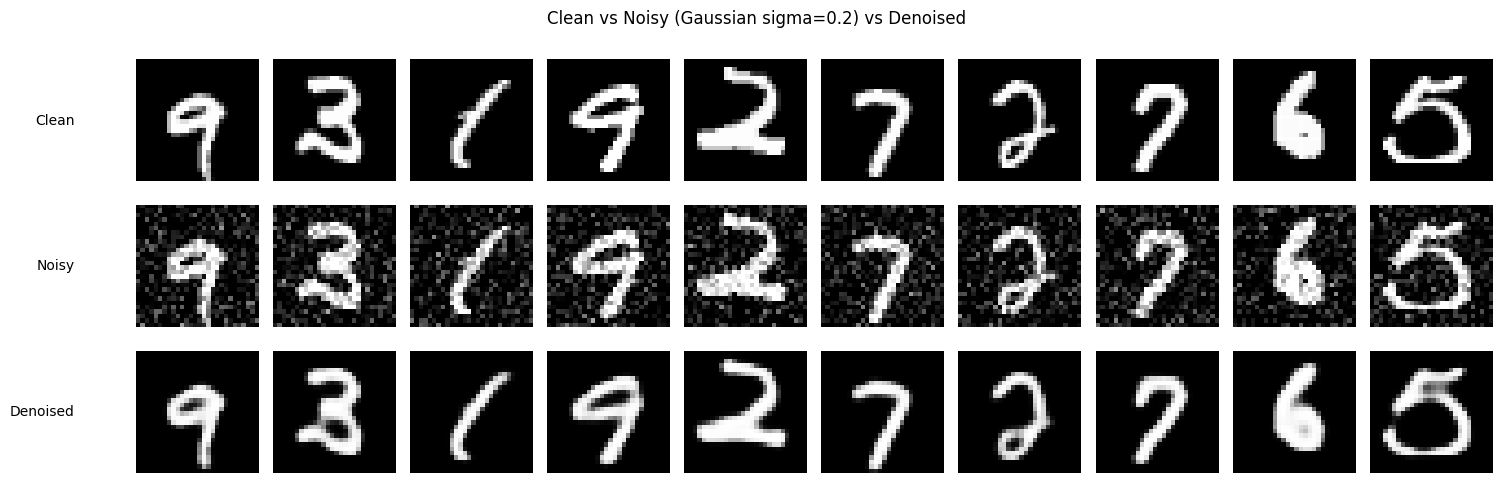
\includegraphics[width=0.9\linewidth]{images/plot4.png}
\caption{Clean versus noisy (Gaussian $\sigma=0.2$) versus denoised test images.}
\label{fig:plot4}
\end{figure}

\begin{figure}[H]
\centering
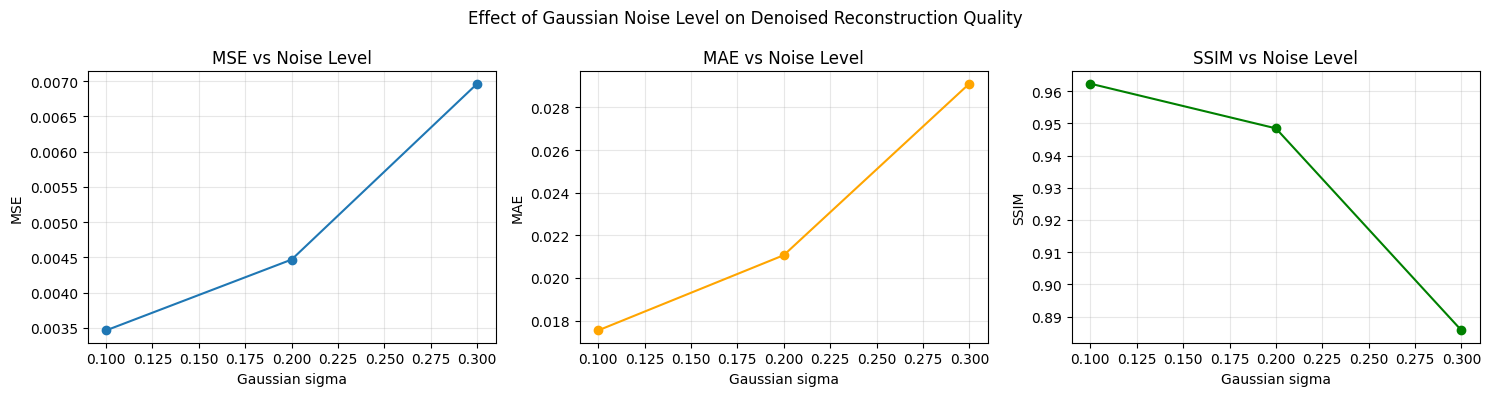
\includegraphics[width=0.95\linewidth]{images/plot5.png}
\caption{Effect of Gaussian noise level on denoised reconstruction quality (MSE, MAE, SSIM).}
\label{fig:plot5}
\end{figure}

\begin{center}
\begin{tabular}{|l|r|r|r|}
\hline
\textbf{Noise Level ($\sigma$)} & \textbf{MSE} & \textbf{MAE} & \textbf{SSIM}\\
\hline
0.1 & 0.003462 & 0.017543 & 0.962333\\
0.2 & 0.004468 & 0.021070 & 0.948457\\
0.3 & 0.006966 & 0.029112 & 0.885719\\
\hline
\end{tabular}
\end{center}

\begin{center}
\begin{tabular}{|l|r|r|r|}
\hline
\textbf{Salt-Pepper Level ($p$)} & \textbf{MSE} & \textbf{MAE} & \textbf{SSIM}\\
\hline
0.05 & 0.004757 & 0.021012 & 0.934433\\
0.10 & 0.006981 & 0.027018 & 0.888367\\
0.20 & 0.013783 & 0.043147 & 0.767158\\
\hline
\end{tabular}
\end{center}

As the Gaussian noise level increases from $\sigma=0.1$ to $\sigma=0.3$, MSE and MAE roughly double while
SSIM drops from 0.962 to 0.886. The model, trained only at $\sigma=0.2$, still generalizes reasonably to
nearby noise levels but degrades faster outside its training level, and is evaluated here on
salt-and-pepper noise it never saw during training -- its SSIM still declines with increasing
corruption ($p=0.05\to0.20$: SSIM $0.934\to0.767$), confirming that the model recovers major digit
structure under both noise types but loses fine detail as corruption grows more severe.

%%%%%%%%%%%%%%%%%%%%%%%%%%%%%%%%%%%%%%%%%%%%%%%%%%%%%%%%%%%%
\section{Variational Autoencoder}
%%%%%%%%%%%%%%%%%%%%%%%%%%%%%%%%%%%%%%%%%%%%%%%%%%%%%%%%%%%%

A conventional autoencoder maps an input to a deterministic latent vector $z=f(x)$. A VAE instead learns
a distribution $q_\phi(z|x) = \mathcal{N}(\mu(x), \mathrm{diag}(\sigma^2(x)))$. The encoder outputs
$\mu, \log\sigma^2$, and a latent vector is drawn using the reparameterization trick
$z = \mu + \sigma \odot \epsilon,\ \epsilon\sim\mathcal{N}(0,I)$, which keeps the sampling step
differentiable with respect to the encoder parameters.

%%%%%%%%%%%%%%%%%%%%%%%%%%%%%%%%%%%%%%%%%%%%%%%%%%%%%%%%%%%%
\section{VAE Loss Function}
%%%%%%%%%%%%%%%%%%%%%%%%%%%%%%%%%%%%%%%%%%%%%%%%%%%%%%%%%%%%

The VAE objective combines a Binary Cross-Entropy reconstruction term with the closed-form KL divergence
against the standard normal prior $p(z)=\mathcal{N}(0,I)$:
\[
D_{KL}\big(q_\phi(z|x)\,\|\,p(z)\big) = -\frac{1}{2}\sum_j \left(1+\log\sigma_j^2-\mu_j^2-\sigma_j^2\right),
\qquad \mathcal{L}_{VAE} = \mathcal{L}_{rec} + \mathcal{L}_{KL}.
\]

%%%%%%%%%%%%%%%%%%%%%%%%%%%%%%%%%%%%%%%%%%%%%%%%%%%%%%%%%%%%
\section{VAE Implementation}
%%%%%%%%%%%%%%%%%%%%%%%%%%%%%%%%%%%%%%%%%%%%%%%%%%%%%%%%%%%%

A compact convolutional encoder/decoder was used with a 2-dimensional latent space (chosen for direct
visualization). The encoder produces $\mu,\log\sigma^2 \in \mathbb{R}^2$; the decoder maps
$z\in\mathbb{R}^2$ back to a $28\times28\times1$ image via dense and transposed-convolution layers. The
model (encoder $+$ decoder) has 284{,}933 trainable parameters and was trained for 30 epochs (Adam,
$\eta=10^{-3}$), taking 32.42 s.

\begin{figure}[H]
\centering
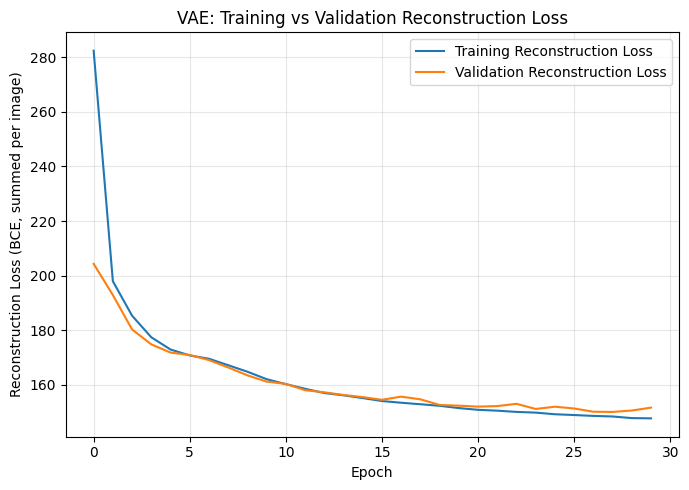
\includegraphics[width=0.65\linewidth]{images/plot9.png}
\caption{VAE training versus validation reconstruction loss (summed BCE per image).}
\label{fig:plot9}
\end{figure}

Both curves fall sharply in the first few epochs and then flatten, with validation loss tracking training
loss closely throughout (final training reconstruction loss 147.67, final validation reconstruction loss
151.61), indicating stable convergence without significant overfitting.

\begin{center}
\begin{tabular}{|l|r|}
\hline
\textbf{VAE Metric} & \textbf{Value}\\
\hline
Reconstruction Loss (val) & 151.6052\\
KL Loss (val) & 6.2382\\
Total Loss (val) & 157.8434\\
Test MSE & 0.044460\\
Test MAE & 0.101560\\
Mean SSIM & 0.516786\\
\hline
\end{tabular}
\end{center}

The VAE's reconstruction metrics (MSE, SSIM) are visibly weaker than the deterministic CAE's, which is
expected: compressing all digit variation into only 2 latent dimensions, combined with the KL penalty
that regularizes the latent space toward $\mathcal{N}(0,I)$, trades reconstruction sharpness for a smooth,
generative latent space.

%%%%%%%%%%%%%%%%%%%%%%%%%%%%%%%%%%%%%%%%%%%%%%%%%%%%%%%%%%%%
\section{Exploring the VAE Latent Space}
%%%%%%%%%%%%%%%%%%%%%%%%%%%%%%%%%%%%%%%%%%%%%%%%%%%%%%%%%%%%

\begin{figure}[H]
\centering
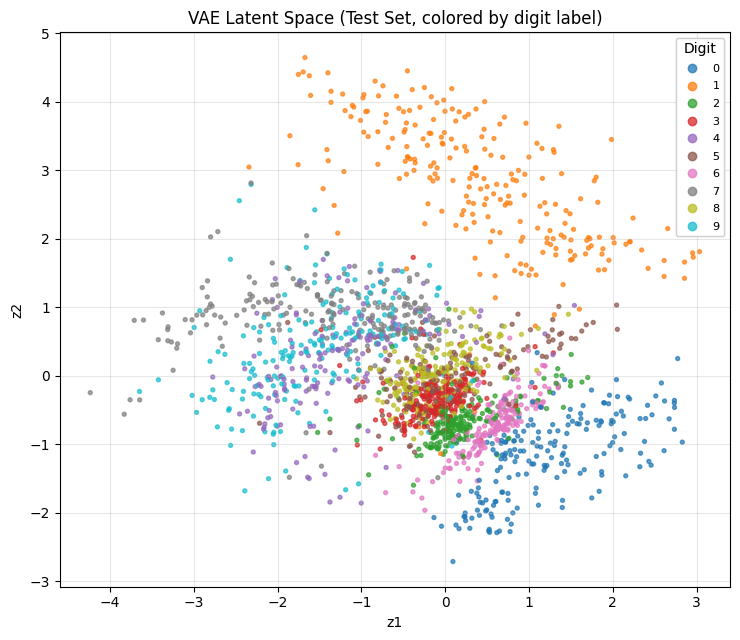
\includegraphics[width=0.62\linewidth]{images/plot6.png}
\caption{VAE latent space ($z_1,z_2$) of the test set, colored by digit label (labels used only for visualization).}
\label{fig:plot6}
\end{figure}

The encoded test points ($z_{\text{mean}}$ range: $x\in[-4.23,3.04]$, $y\in[-2.71,4.65]$) form
recognizable clusters: digit 1 occupies a distinct region at high $z_2$, digit 0 separates toward
positive $z_1$/negative $z_2$, and 3, 4, 5, 8 overlap heavily near the origin because these digits share
similar curved-stroke structure that a 2-D bottleneck cannot fully disentangle. The overlap in the dense
central region is consistent with the VAE's comparatively lower SSIM, since visually similar digits are
mapped to nearby latent codes and become harder for the decoder to reconstruct unambiguously.

%%%%%%%%%%%%%%%%%%%%%%%%%%%%%%%%%%%%%%%%%%%%%%%%%%%%%%%%%%%%
\section{Generating New Images with the VAE}
%%%%%%%%%%%%%%%%%%%%%%%%%%%%%%%%%%%%%%%%%%%%%%%%%%%%%%%%%%%%

\begin{figure}[H]
\centering
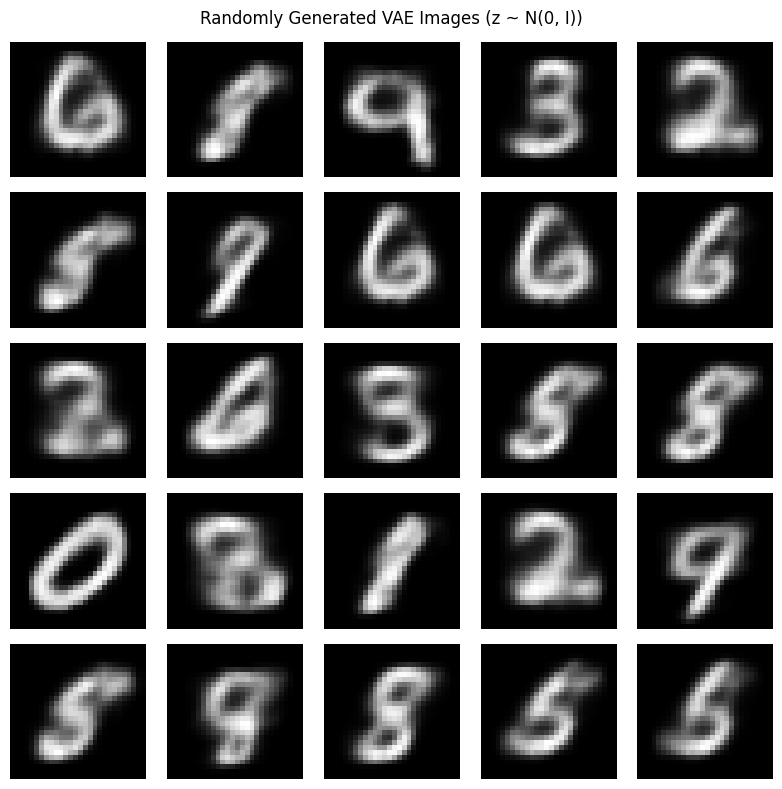
\includegraphics[width=0.55\linewidth]{images/plot7.png}
\caption{25 images generated by sampling $z\sim\mathcal{N}
\label{fig:plot7}(0,I)$ and decoding.}
\end{figure}

Many of the generated samples are clearly recognizable as digits (6, 9, 3, 2, 0 are legible), confirming
that the decoder has learned a meaningful generative mapping from the prior. There is visible variation
in stroke style and digit identity across the grid, but several samples are blurred or ambiguous between
two digits (e.g.\ shapes between 5 and 6, or 3 and 8) -- a direct consequence of the overlapping latent
regions seen in Figure~\ref{fig:plot6} and the limited capacity of a 2-D latent space.

%%%%%%%%%%%%%%%%%%%%%%%%%%%%%%%%%%%%%%%%%%%%%%%%%%%%%%%%%%%%
\section{Latent Space Interpolation}
%%%%%%%%%%%%%%%%%%%%%%%%%%%%%%%%%%%%%%%%%%%%%%%%%%%%%%%%%%%%

\begin{figure}[H]
\centering
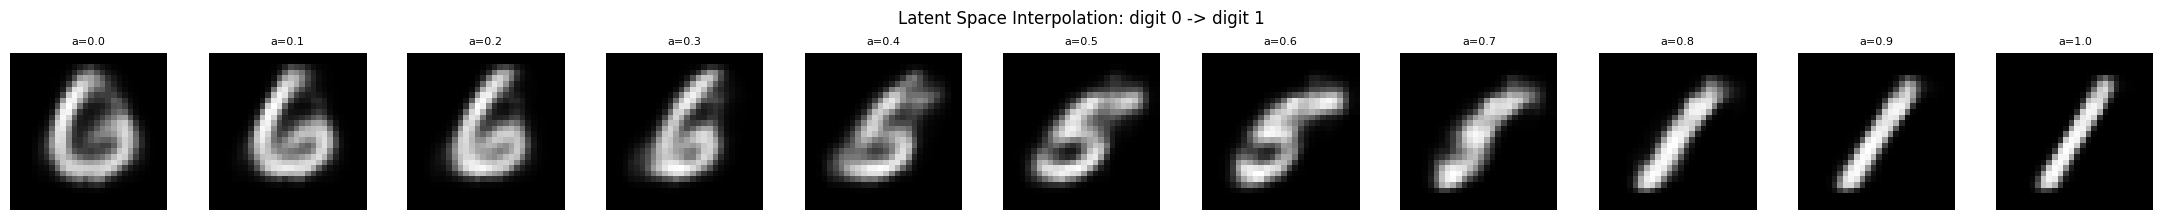
\includegraphics[width=\linewidth]{images/plot8.png}
\caption{Decoded images along the linear interpolation $z(\alpha)=(1-\alpha)z_A+\alpha z_B$ between a digit-0 and a digit-1 latent code, $\alpha=0,0.1,\dots,1.0$.}
\label{fig:plot8}
\end{figure}

The decoded image changes smoothly and continuously as $\alpha$ increases: the initial frames resemble a
6-like loop (reflecting the chosen test sample's z-position rather than a clean 0), passing through a
5-like intermediate shape before straightening into a 1 by $\alpha=0.8$--$1.0$. No abrupt jumps or
discontinuities appear, demonstrating that the VAE's latent space is locally continuous and semantically
organized.

%%%%%%%%%%%%%%%%%%%%%%%%%%%%%%%%%%%%%%%%%%%%%%%%%%%%%%%%%%%%
\section{Reconstruction Comparison Across Models}
%%%%%%%%%%%%%%%%%%%%%%%%%%%%%%%%%%%%%%%%%%%%%%%%%%%%%%%%%%%%

\begin{center}
\begin{tabular}{|l|r|r|r|r|}
\hline
\textbf{Model} & \textbf{MSE} & \textbf{MAE} & \textbf{SSIM} & \textbf{Parameters}\\
\hline
Fully Connected AE & 0.02227 & 0.05919 & 0.74599 & 211{,}040\\
Convolutional AE & 0.00242 & 0.01471 & 0.97535 & 74{,}497\\
Denoising CAE & 0.00447 & 0.02107 & 0.94846 & 74{,}497\\
\hline
\end{tabular}
\end{center}

\begin{center}
\begin{tabular}{|l|r|}
\hline
\textbf{VAE Metric} & \textbf{Value}\\
\hline
Reconstruction Loss & 151.6052\\
KL Loss & 6.2382\\
Total Loss & 157.8434\\
Test MSE & 0.044460\\
Test MAE & 0.101560\\
Mean SSIM & 0.516786\\
\hline
\end{tabular}
\end{center}

%%%%%%%%%%%%%%%%%%%%%%%%%%%%%%%%%%%%%%%%%%%%%%%%%%%%%%%%%%%%
\section{Reconstruction Error Distribution}
%%%%%%%%%%%%%%%%%%%%%%%%%%%%%%%%%%%%%%%%%%%%%%%%%%%%%%%%%%%%

Per-image reconstruction error $e_i = \frac{1}{D}\sum_j (x_{ij}-\hat{x}_{ij})^2$ was computed on the CAE
test-set reconstructions.

\begin{figure}[H]
\centering
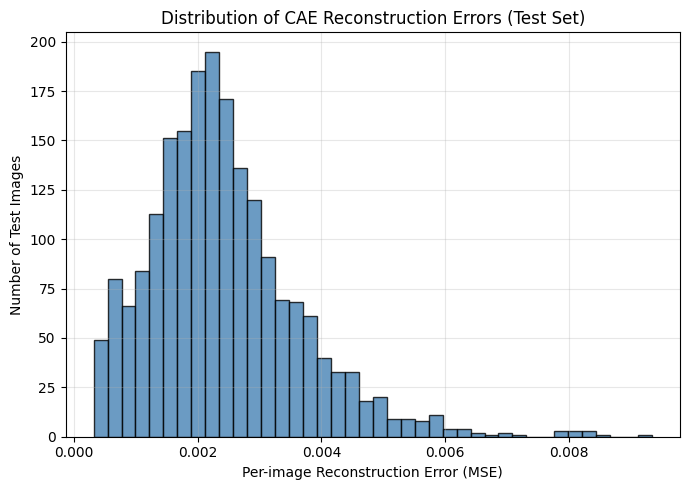
\includegraphics[width=0.65\linewidth]{images/plot10.png}
\caption{Distribution of per-image CAE reconstruction errors on the test set.}
\label{fig:plot10}
\end{figure}

\begin{center}
\begin{tabular}{|l|r|}
\hline
\textbf{Statistic} & \textbf{Value}\\
\hline
Minimum error & 0.000313\\
Maximum error & 0.009349\\
Mean error & 0.002419\\
Median error & 0.002256\\
90th percentile & 0.003957\\
95th percentile & 0.004605\\
99th percentile & 0.006195\\
\hline
\end{tabular}
\end{center}

The distribution is unimodal and right-skewed, concentrated between roughly 0.0005 and 0.004 with a long
thin tail extending to about 0.0093. The bulk of test images are reconstructed very accurately (median
0.00226), while a small minority of harder, atypically-drawn samples drive the tail.

%%%%%%%%%%%%%%%%%%%%%%%%%%%%%%%%%%%%%%%%%%%%%%%%%%%%%%%%%%%%
\section{Required High-Error Image Analysis}
%%%%%%%%%%%%%%%%%%%%%%%%%%%%%%%%%%%%%%%%%%%%%%%%%%%%%%%%%%%%

\begin{figure}[H]
\centering
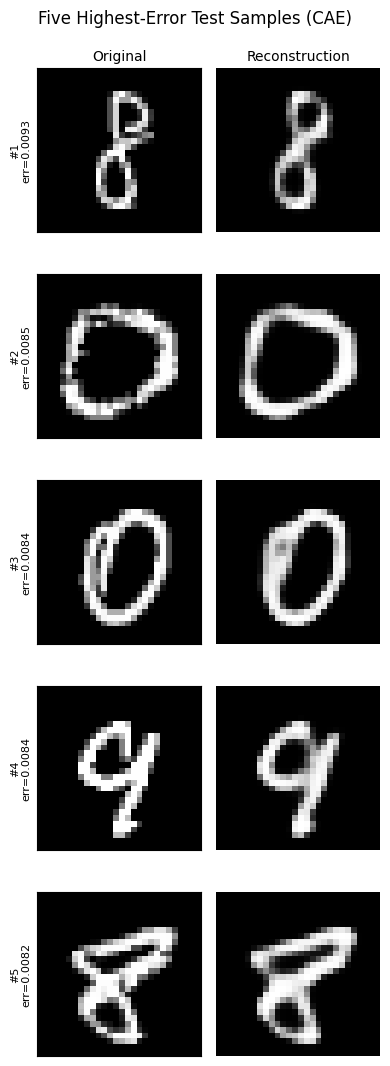
\includegraphics[width=0.32\linewidth]{images/high_error_samples.png}
\caption{Five highest-error CAE test samples: original (left) versus reconstruction (right).}
\label{fig:higherror}
\end{figure}

\begin{center}
\begin{tabular}{|c|c|c|r|}
\hline
\textbf{Rank} & \textbf{Test Index} & \textbf{True Digit} & \textbf{MSE}\\
\hline
1 & 589 & 8 & 0.009349\\
2 & 1317 & 0 & 0.008477\\
3 & 434 & 0 & 0.008397\\
4 & 949 & 9 & 0.008377\\
5 & 152 & 8 & 0.008226\\
\hline
\end{tabular}
\end{center}

Four of the five hardest samples are 0s and 8s, drawn with unusually thick strokes, tight loops or an
open/closed ambiguity (e.g.\ an 8 with a nearly closed lower loop resembling a 0). Such heavy, atypical
stroke widths sit further from the bulk of the training distribution, so the encoder's compressed
representation loses more of the fine loop geometry, producing visibly thinner or slightly misshapen
reconstructions.

%%%%%%%%%%%%%%%%%%%%%%%%%%%%%%%%%%%%%%%%%%%%%%%%%%%%%%%%%%%%
\section{Consolidated Results}
%%%%%%%%%%%%%%%%%%%%%%%%%%%%%%%%%%%%%%%%%%%%%%%%%%%%%%%%%%%%

\begin{center}
\begin{tabular}{|l|r|r|r|r|r|}
\hline
\textbf{Model} & \textbf{MSE} & \textbf{MAE} & \textbf{SSIM} & \textbf{Parameters} & \textbf{Time (s)}\\
\hline
FC Autoencoder & 0.02227 & 0.05919 & 0.74599 & 211{,}040 & 13.61\\
Conv.\ Autoencoder & 0.00242 & 0.01471 & 0.97535 & 74{,}497 & 24.31\\
Denoising CAE & 0.00447 & 0.02107 & 0.94846 & 74{,}497 & 20.41\\
VAE & 0.04446 & 0.10156 & 0.51679 & 284{,}933 & 32.42\\
\hline
\end{tabular}
\end{center}

The Convolutional Autoencoder achieved the best pure reconstruction quality among all four models,
followed by the Denoising CAE (evaluated on noisy inputs), the FC-AE, and finally the VAE, whose latent
space is deliberately regularized for generation rather than optimized purely for reconstruction fidelity.

%%%%%%%%%%%%%%%%%%%%%%%%%%%%%%%%%%%%%%%%%%%%%%%%%%%%%%%%%%%%
\section{Additional Latent-Dimension Study}
%%%%%%%%%%%%%%%%%%%%%%%%%%%%%%%%%%%%%%%%%%%%%%%%%%%%%%%%%%%%

The fully connected autoencoder was retrained with latent dimensions 2, 8, 16 and 32 (20 epochs each,
identical protocol).

\begin{center}
\begin{tabular}{|c|r|r|r|r|}
\hline
\textbf{Latent Dim} & \textbf{MSE} & \textbf{SSIM} & \textbf{Parameters} & \textbf{Time (s)}\\
\hline
2 & 0.04718 & 0.47048 & 210{,}130 & 12.50\\
8 & 0.02756 & 0.69317 & 210{,}520 & 11.67\\
16 & 0.02091 & 0.76230 & 211{,}040 & 11.15\\
32 & 0.01837 & 0.79033 & 212{,}080 & 13.33\\
\hline
\end{tabular}
\end{center}

\begin{figure}[H]
\centering
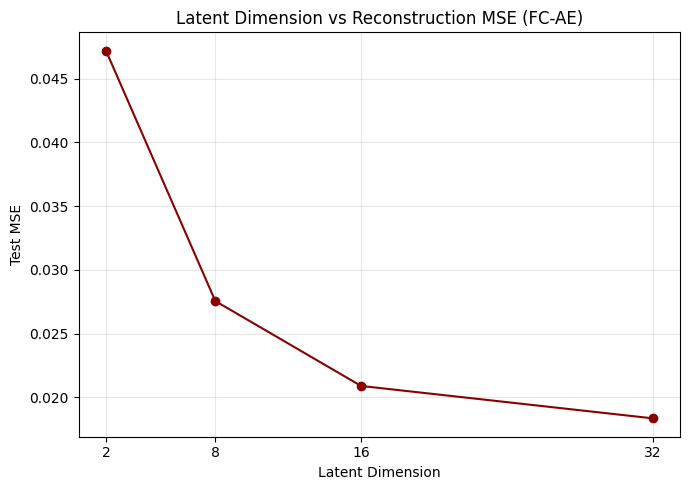
\includegraphics[width=0.62\linewidth]{images/plot11.png}
\caption{Latent dimension versus test-set reconstruction MSE for the FC-AE.}
\label{fig:plot11}
\end{figure}

MSE decreases and SSIM increases monotonically as the latent dimension grows from 2 to 32, but with
diminishing returns: the largest single improvement is between dim 2 and dim 8 (MSE $0.047\to0.028$),
while the gain from 16 to 32 is comparatively small (MSE $0.021\to0.018$). This illustrates the classic
compression-versus-quality trade-off -- a larger bottleneck retains more information and reconstructs
better, but the marginal benefit shrinks once the latent space is large enough to capture most of the
digit variation.

%%%%%%%%%%%%%%%%%%%%%%%%%%%%%%%%%%%%%%%%%%%%%%%%%%%%%%%%%%%%
\section{Required Plots}
%%%%%%%%%%%%%%%%%%%%%%%%%%%%%%%%%%%%%%%%%%%%%%%%%%%%%%%%%%%%

All plots required by the experiment specification (original vs.\ reconstructed, training/validation
loss, FC-AE vs.\ CAE, clean/noisy/denoised, noise level vs.\ metrics, VAE latent space, generated
samples, latent interpolation, VAE training/validation loss, and the reconstruction-error distribution)
are presented in the corresponding sections above (Figures 1--10), each with its own inference discussing
what the plot shows, the trend observed, why the trend likely occurs, and the conclusion drawn from it.

%%%%%%%%%%%%%%%%%%%%%%%%%%%%%%%%%%%%%%%%%%%%%%%%%%%%%%%%%%%%
\section{Required Inferences}
%%%%%%%%%%%%%%%%%%%%%%%%%%%%%%%%%%%%%%%%%%%%%%%%%%%%%%%%%%%%

\begin{itemize}
\item \textbf{Effect of latent dimension on reconstruction:} MSE falls and SSIM rises monotonically from
dim 2 to dim 32 (Table in Sec.~25), with diminishing gains at larger sizes -- larger bottlenecks retain
more digit information but returns saturate once most variance is captured.
\item \textbf{FC vs.\ convolutional reconstruction:} the CAE outperforms the FC-AE on every metric while
using fewer parameters, because convolution preserves 2-D spatial locality that flattening destroys.
\item \textbf{Effect of Gaussian noise level:} SSIM falls from 0.962 to 0.886 as $\sigma$ rises from 0.1
to 0.3; larger corruption removes more true signal, so the denoiser has less to work with.
\item \textbf{Denoising autoencoder's ability to recover structure:} even at the highest tested noise
levels the digit outline remains recognizable in Figure~\ref{fig:plot4}, showing the model recovers global structure
better than fine strokes.
\item \textbf{VAE latent distribution characteristics:} the encoder produces smoothly varying $\mu,
\log\sigma^2$ values that keep the aggregate posterior close to $\mathcal{N}(0,I)$, evidenced by the KL
loss stabilizing near 6.2 rather than growing unbounded.
\item \textbf{Structure of the 2-D VAE latent space:} distinct digits form loosely separated clusters
with substantial overlap near the origin (Figure~\ref{fig:plot6}), reflecting genuine visual similarity between digits
such as 3/5/8.
\item \textbf{Quality and diversity of generated samples:} most of the 25 generated digits in Figure~\ref{fig:plot7}
are recognizable and show real stylistic variation, though a few fall in ambiguous latent regions and
look intermediate between two digits.
\item \textbf{Smoothness of latent interpolation:} Figure~\ref{fig:plot8} shows a continuous, gradual shape change with
no discontinuities between the two endpoint digits.
\item \textbf{Reconstruction error vs.\ visual quality:} the five highest-error samples (Sec.~16) are
visibly atypical (unusually thick or ambiguous strokes), directly linking numerical error to perceptual
difficulty.
\item \textbf{Deterministic vs.\ probabilistic latent representations:} the CAE's deterministic code
achieves far higher SSIM (0.975) than the VAE's probabilistic code (0.517) at comparable capacity,
because the VAE trades reconstruction sharpness for a smooth, continuous, generative latent space.
\end{itemize}

%%%%%%%%%%%%%%%%%%%%%%%%%%%%%%%%%%%%%%%%%%%%%%%%%%%%%%%%%%%%
\section{Discussion Questions}
%%%%%%%%%%%%%%%%%%%%%%%%%%%%%%%%%%%%%%%%%%%%%%%%%%%%%%%%%%%%

\begin{enumerate}[label=\arabic*.]
\item \textbf{What is an autoencoder?} A neural network trained to reconstruct its own input through a
compressed intermediate (latent) representation, learning efficient encodings without labels.

\item \textbf{Purpose of the encoder?} Compresses the input into a lower-dimensional latent vector that
retains the information needed to reconstruct the image.

\item \textbf{Purpose of the decoder?} Maps the latent vector back to the original input space,
reconstructing an approximation of the input image.

\item \textbf{What is a latent representation?} A compact, lower-dimensional vector $z$ that summarizes
the essential content of the input, produced by the encoder.

\item \textbf{Why is the latent representation usually smaller than the input?} To force the network to
learn a compressed, non-trivial encoding rather than simply copying the input through.

\item \textbf{What happens when the latent dimension is too small?} Reconstruction quality degrades
(higher MSE, lower SSIM) because too little information can pass through the bottleneck, as seen at
dim=2 (MSE 0.047).

\item \textbf{What happens when the latent dimension is increased?} Reconstruction quality improves with
diminishing returns, since more capacity is available to retain fine detail, up to a saturation point.

\item \textbf{Why can a CAE preserve spatial information more effectively?} Convolutional filters operate
locally and share weights across spatial positions, preserving 2-D structure that a fully-connected
flatten operation destroys.

\item \textbf{Differentiate an autoencoder and a denoising autoencoder.} A plain autoencoder reconstructs
its own clean input; a denoising autoencoder receives a corrupted input but is trained against the clean
target, forcing it to learn noise-robust features.

\item \textbf{Why is the clean image used as the target in denoising?} So the network learns to recover
the true underlying signal rather than simply copying the corrupted input.

\item \textbf{What happens when the noise level is increased?} Reconstruction quality worsens
monotonically (SSIM fell from 0.962 to 0.886 as $\sigma$ rose from 0.1 to 0.3), since more true signal is
destroyed.

\item \textbf{Why are MSE, MAE and SSIM useful for image reconstruction?} MSE/MAE quantify pixel-level
error magnitude, while SSIM captures perceptual/structural similarity, so together they give both a
numerical and a visually meaningful measure of quality.

\item \textbf{What is a Variational Autoencoder?} An autoencoder that learns a probability distribution
over the latent space instead of a single deterministic vector, enabling generation of new samples.

\item \textbf{How does a VAE differ from a conventional autoencoder?} It encodes inputs as a distribution
$(\mu,\log\sigma^2)$ and samples from it, and its loss adds a KL-divergence regularizer to the prior.

\item \textbf{Why does a VAE learn a distribution instead of a single latent vector?} A distribution
makes the latent space continuous and generative, allowing new, unseen points to decode into plausible
images.

\item \textbf{What is the reparameterization trick?} Writing $z=\mu+\sigma\odot\epsilon$ with
$\epsilon\sim\mathcal{N}(0,I)$ so gradients can flow through $\mu,\sigma$ despite the stochastic sampling
step.

\item \textbf{Why is $\epsilon$ sampled from a standard normal distribution?} It provides the external
source of randomness needed for sampling while keeping the transformation to $z$ differentiable in
$\mu,\sigma$.

\item \textbf{Role of KL divergence in the VAE loss?} Regularizes the learned posterior $q_\phi(z|x)$
toward the prior $\mathcal{N}(0,I)$, keeping the latent space smooth, continuous and suitable for
sampling.

\item \textbf{What is the prior distribution used in the VAE?} The standard normal distribution
$p(z)=\mathcal{N}(0,I)$.

\item \textbf{Why is a 2-D latent space useful for visualization?} It can be plotted directly on a 2-D
scatter plot, allowing the cluster structure and digit relationships to be inspected visually, as in
Figure~\ref{fig:plot6}.

\item \textbf{What does latent-space interpolation demonstrate?} That the latent space is continuous and
semantically organized, since intermediate points decode into plausible in-between images (Figure~\ref{fig:plot8}).

\item \textbf{Why can a VAE generate new images?} Because its prior $\mathcal{N}(0,I)$ covers the entire
latent space with a known, simple distribution, any sampled point can be decoded into a plausible image.

\item \textbf{Why might some VAE-generated images be unclear?} They may fall in overlapping latent
regions shared by multiple digit classes (Figure~\ref{fig:plot6}), producing decoded images that blend features of two
digits.

\item \textbf{Difference between reconstruction and generation?} Reconstruction decodes the latent code
of a real, encoded input; generation decodes an arbitrary latent code sampled from the prior, with no
corresponding real input.

\item \textbf{Why should test images remain unseen during training?} To obtain an unbiased estimate of
how well the model generalizes to new data rather than measuring memorization of the training set.
\end{enumerate}

%%%%%%%%%%%%%%%%%%%%%%%%%%%%%%%%%%%%%%%%%%%%%%%%%%%%%%%%%%%%
\section{Additional Exercises}
%%%%%%%%%%%%%%%%%%%%%%%%%%%%%%%%%%%%%%%%%%%%%%%%%%%%%%%%%%%%

\textbf{Exercise 1 -- CAE with latent channels 4/8/16/32 (10 epochs each):} SSIM rose steadily with
capacity (0.940, 0.955, 0.961, 0.965) and MSE fell (0.00617$\to$0.00355), confirming that a wider
convolutional bottleneck retains more spatial detail, though gains shrink beyond 16 channels.

\textbf{Exercise 2 -- Gaussian vs.\ salt-and-pepper denoising (15 epochs, same architecture):} Gaussian
noise ($\sigma=0.2$) gave MSE 0.00469/SSIM 0.946; salt-and-pepper ($p=0.10$) gave MSE 0.00513/SSIM 0.944
-- comparable difficulty overall, with salt-and-pepper very slightly harder at this configuration.

\textbf{Exercise 3 -- Denoising at two noise levels (15 epochs):} SSIM was 0.962 at $\sigma=0.1$ versus
0.917 at $\sigma=0.3$ when each model was trained and tested at its own noise level, confirming that
higher corruption consistently lowers achievable reconstruction quality.

\textbf{Exercise 4 -- Conv2DTranspose vs.\ UpSampling2D decoder (20 epochs):} Conv2DTranspose slightly
outperformed UpSampling2D (SSIM 0.978 vs.\ 0.975, MSE 0.00209 vs.\ 0.00242) at the cost of more
parameters (111{,}425 vs.\ 74{,}497), since learned transposed-convolution kernels can recover detail
that fixed upsampling cannot.

\textbf{Exercise 5 -- VAE latent dim 2 vs.\ 8 (20 epochs):} increasing the latent dimension from 2 to 8
substantially improved reconstruction (SSIM 0.517$\to$0.778, MSE 0.0445$\to$0.0208), showing that 2-D
latent capacity is the main bottleneck limiting VAE reconstruction quality.

\textbf{Exercise 6 -- Effect of KL weight $\beta$ (20 epochs):} at $\beta=0.5,1.0,5.0$ the KL loss fell
(6.57, 5.60, 3.43) while reconstruction loss rose slightly and SSIM dropped marginally (0.494, 0.496,
0.469) -- a larger $\beta$ compresses the latent space more aggressively toward the prior, trading
reconstruction fidelity for a more regularized latent space.

\textbf{Exercise 7 -- Larger 10$\times$10 generated grid:} the mean per-pixel standard deviation across
100 generated samples was 0.1160, confirming meaningful pixel-level diversity rather than the decoder
collapsing to near-identical outputs.

\textbf{Exercise 8 -- Interpolation between digit 3 and digit 8 latent regions:} the decoded sequence
changed smoothly across all 11 interpolation steps (see \texttt{exercise8\_interpolation.png}), reaffirming
the latent space's local continuity for a second, independent digit pair.

\begin{figure}[H]
\centering
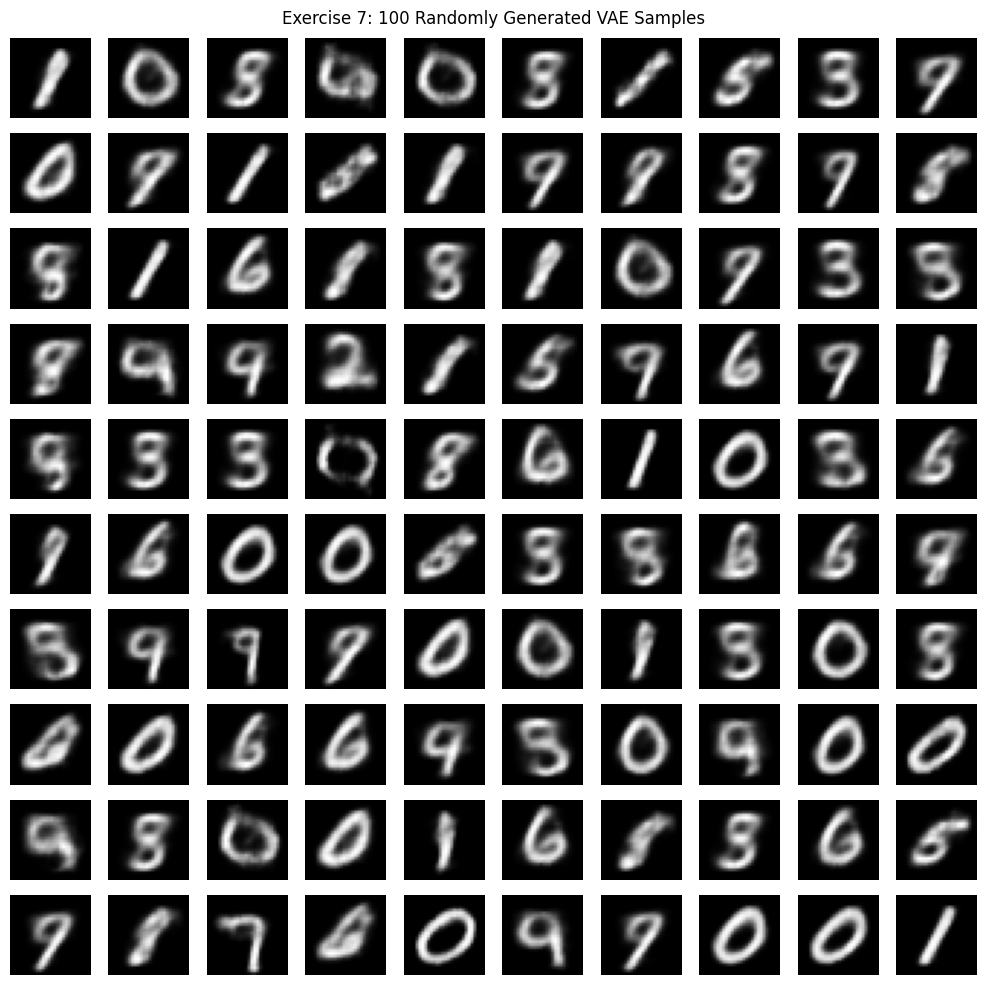
\includegraphics[width=0.75\linewidth]{images/exercise7_large_grid.png}
\caption{Exercise 7: 100 randomly generated VAE samples ($z\sim\mathcal{N}
\label{fig:ex7}(0,I)$).}
\end{figure}

\begin{figure}[H]
\centering
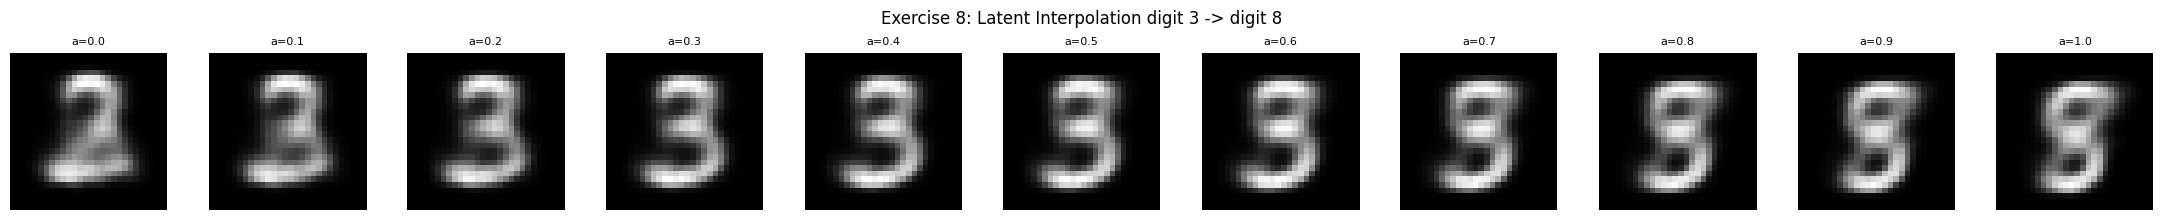
\includegraphics[width=\linewidth]{images/exercise8_interpolation.png}
\caption{Exercise 8: latent-space interpolation between a digit-3 and a digit-8 test sample.}
\label{fig:ex8}
\end{figure}

%%%%%%%%%%%%%%%%%%%%%%%%%%%%%%%%%%%%%%%%%%%%%%%%%%%%%%%%%%%%
\section{Expected Outcome}
%%%%%%%%%%%%%%%%%%%%%%%%%%%%%%%%%%%%%%%%%%%%%%%%%%%%%%%%%%%%

The completed pipeline demonstrates the full image-representation and reconstruction workflow
(Image $\to$ Encoder $\to$ Latent Representation $\to$ Decoder $\to$ Reconstructed Image), the denoising
workflow (Clean Image $\to$ Noise $\to$ Denoising Autoencoder $\to$ Recovered Image), and the variational
generative workflow (Image $\to (\mu,\sigma) \to z \to$ Decoder $\to$ Generated/Reconstructed Image), each
supported by quantitative evaluation (MSE, MAE, SSIM) and visual analysis obtained from the student's own
execution.

%%%%%%%%%%%%%%%%%%%%%%%%%%%%%%%%%%%%%%%%%%%%%%%%%%%%%%%%%%%%
\section{Conclusion}
%%%%%%%%%%%%%%%%%%%%%%%%%%%%%%%%%%%%%%%%%%%%%%%%%%%%%%%%%%%%

This experiment implemented and compared four autoencoder variants on a 10,000/2,000-image MNIST subset.
The FC-AE (latent 16) reached test MSE 0.0223 / SSIM 0.746, while the CAE achieved substantially better
reconstruction (MSE 0.0024, SSIM 0.975) with fewer parameters, confirming that preserving spatial
structure through convolution is more effective than flattening. The denoising CAE, trained on Gaussian
noise ($\sigma=0.2$), reached SSIM 0.948 and degraded predictably as noise increased, recovering global
digit structure even under stronger corruption. The VAE (2-D latent) reached reconstruction loss 151.6,
KL loss 6.24, MSE 0.0445 and SSIM 0.517 -- lower reconstruction fidelity than the deterministic models,
but its regularized latent space produced a smoothly clustered visualization, recognizable generated
digits, and continuous interpolation between digit pairs. The latent-dimension study showed reconstruction
quality improving monotonically with capacity with diminishing returns beyond dimension 16. Across all
eight additional exercises, wider convolutional bottlenecks, transposed-convolution decoders, and larger
VAE latent spaces consistently improved reconstruction quality, while increasing the KL weight traded
reconstruction sharpness for stronger latent regularization. Overall, the results confirm that
deterministic convolutional autoencoders are best suited for pure reconstruction, while VAEs trade some
reconstruction accuracy for a structured, generative latent space.

%%%%%%%%%%%%%%%%%%%%%%%%%%%%%%%%%%%%%%%%%%%%%%%%%%%%%%%%%%%%
\section{Source Code}
%%%%%%%%%%%%%%%%%%%%%%%%%%%%%%%%%%%%%%%%%%%%%%%%%%%%%%%%%%%%

The complete implementation was carried out in Python using Google Colab.

\url{https://github.com/K-Mithran/Deep-Learning/Lab7/DL_7.ipynb}

The complete source code used in this experiment is available in the submitted Google Colab notebook and
GitHub repository.

%%%%%%%%%%%%%%%%%%%%%%%%%%%%%%%%%%%%%%%%%%%%%%%%%%%%%%%%%%%%
\section{References}
%%%%%%%%%%%%%%%%%%%%%%%%%%%%%%%%%%%%%%%%%%%%%%%%%%%%%%%%%%%%

\begin{enumerate}[label=\arabic*.]
\item Ian Goodfellow, Yoshua Bengio and Aaron Courville, \textit{Deep Learning}, MIT Press, 2016.
\item Diederik P. Kingma and Max Welling, ``Auto-Encoding Variational Bayes,'' ICLR, 2014.
\item Pascal Vincent et al., ``Stacked Denoising Autoencoders: Learning Useful Representations in a Deep
Network with a Local Denoising Criterion,'' \textit{Journal of Machine Learning Research}, 2010.
\item Yann LeCun, Corinna Cortes and Christopher J.\ C.\ Burges, ``MNIST Handwritten Digit Database.''
\item TensorFlow Documentation: \url{https://www.tensorflow.org}
\item Keras Documentation: \url{https://keras.io}
\item scikit-image Documentation: \url{https://scikit-image.org}
\end{enumerate}

\end{document}
